\documentclass{standalone}
\usepackage{tikz}
% Show the answer when compiled on its own; the test template's
% \ans shows it only in the answer key
\providecommand{\ans}[1]{#1}
\begin{document}
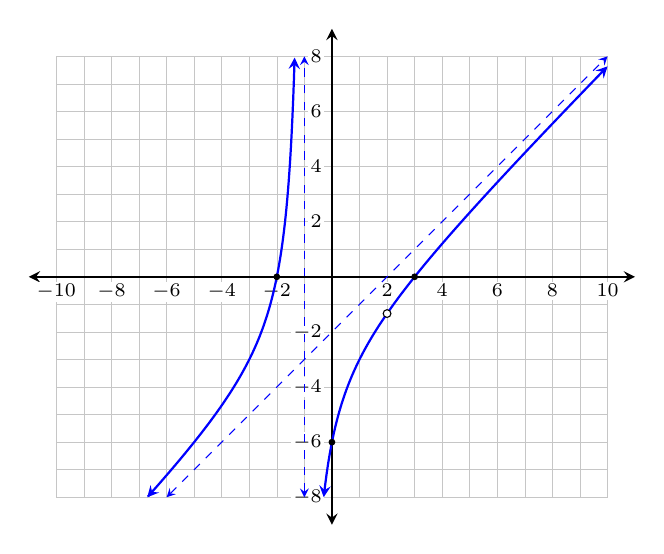
\begin{tikzpicture}[>=stealth, scale=0.35]
  % Same blank grid as 40.tex, with the graph of
  % r(x) = (x - 3)(x + 2) / (x + 1), hole at (2, -4/3)
  \draw[gray!45, very thin] (-10,-8) grid (10,8);
  % Axes and labels drawn before the graph so the label halos
  % never hide part of the curve
  \draw[<->, thick] (-11,0) -- (11,0);
  \draw[<->, thick] (0,-9) -- (0,9);
  \foreach \x in {-10,-8,-6,-4,-2,2,4,6,8,10} {
    \node[below, font=\scriptsize, fill=white, inner sep=1pt] at (\x,-0.15) {$\x$};
  }
  \foreach \y in {-8,-6,-4,-2,2,4,6,8} {
    \node[left, font=\scriptsize, fill=white, inner sep=1pt] at (-0.25,\y) {$\y$};
  }
  % Answer strokes, drawn only in the answer key
  \ans{%
    % Asymptotes: x = -1 and the slant asymptote y = x - 2
    \draw[<->, dashed, blue] (-1,-8) -- (-1,8);
    \draw[<->, dashed, blue] (-6,-8) -- (10,8);
    % Each branch ends where the graph leaves the window (|r| = 8)
    \draw[<->, thick, blue, samples=200, domain=-6.701:-1.353]
      plot (\x, {(\x-3)*(\x+2)/(\x+1)});
    \draw[<->, thick, blue, samples=200, domain=-0.298:10]
      plot (\x, {(\x-3)*(\x+2)/(\x+1)});
    % Zeros, y-intercept, and hole
    \fill[black] (-2,0) circle (3.5pt);
    \fill[black] (3,0) circle (3.5pt);
    \fill[black] (0,-6) circle (3.5pt);
    \draw[fill=white, draw=black] (2,-4/3) circle (4pt);
  }
\end{tikzpicture}
\end{document}
